\documentclass[conference]{article}

% Packages for additional functionality
\usepackage[margin=.75in]{geometry}
\usepackage[utf8]{inputenc}
\usepackage{amsmath, amssymb}
\usepackage{graphicx}
\usepackage{algorithm}
\usepackage{algorithmic}
\usepackage[backend=biber,style=numeric,citestyle=ieee]{biblatex}
\usepackage{pdfpages}
\addbibresource{references.bib}
% \usepackage{cleveref}

\title{\LARGE \bf
Project Abstract
}
\author{
    Jack Vranicar
}
\begin{document}
\maketitle

\thispagestyle{empty}
\pagestyle{empty}

\section{Proposal}
This goal for this project is to characterize the properties of a 3D printed spring. The spring will be printed out of PLA and be made of a single layer. The spring is constructed by joining multiple 'S' shaped sections together. At first, a simple model will be used to predict the behavior of the springs. This model will assume that the bends of the 'S' profiles are the only parts of the spring that move. Therefore, the system can be modeled as a series of 'L' shaped links that are attached to each other with rotational springs and dampers (see Figure \ref{fig:1}).

Furthermore, it will be assumed that every link moves perfectly vertically, such that each angle on the right hand side of the spring is equal, and similarly on the left hand side. Consequently, this means that the angles on the left hand side of the model will be: 
\begin{equation}
\theta_l  = \pi - \theta_r
\end{equation}

 To collect data for this project, a test stand will be created. This test stand will hold the spring in place and measure its vertical displacement as a function of time. The method of capturing this measurement has not been decided yet, but some considerations include Hall Effect sensors and IR distance measuring sensors.

From this project, I hope to learn how reliably spring characteristics can be predicted when using 3D prints. If there is a low uncertainty, I'd like to look into implementing these springs into control systems. This could allow for fine-tuned control of 3D printed mechanisms, something that seems to be a novel approach. This is important because one could easily swap springs out or adjust its parameters if the system is found to be uncontrollable with a certain spring constant, something about the system changes (i.e. mass), etc.

\begin{figure}[H]
    \centering
    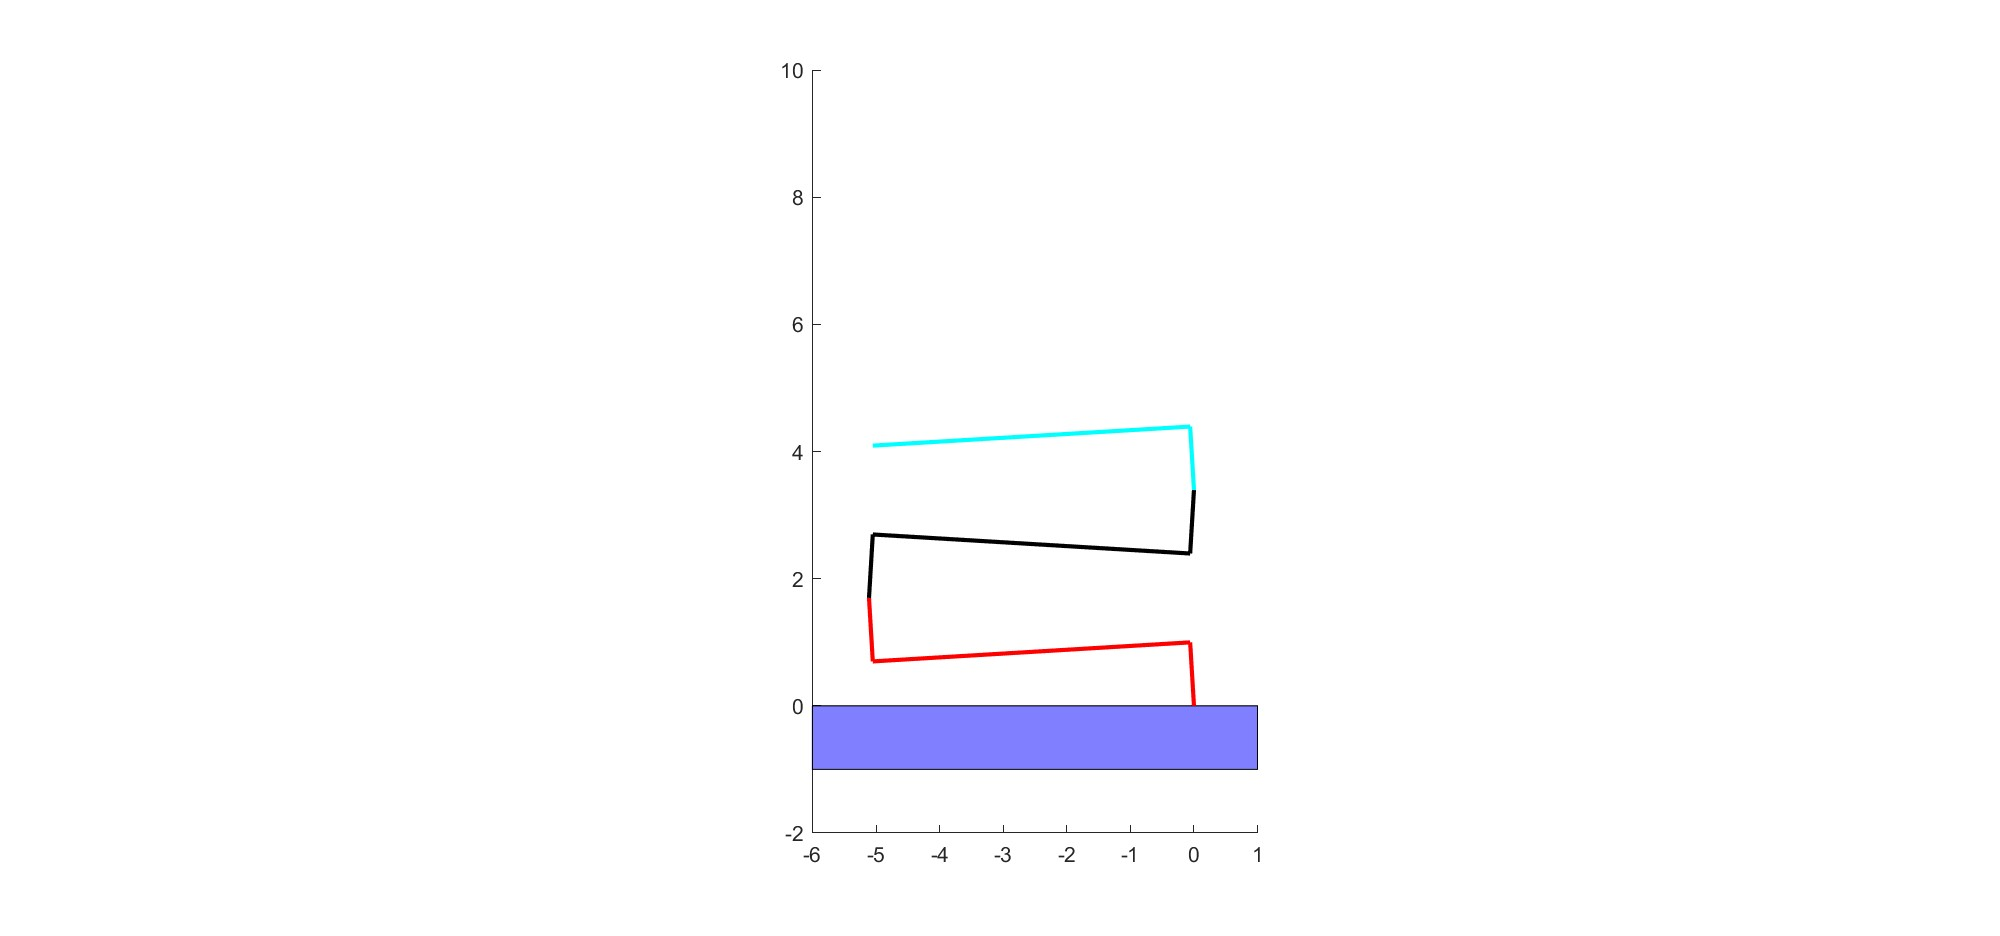
\includegraphics[width=\linewidth]{LinkageExample.jpeg}
    \caption{Spring Model}
    \label{fig:1}
\end{figure}


\newpage
\printbibliography

\end{document}
